\chapter{Processo de alinhamento}

Neste capítulo, será apresentado o processo proposto para alinhar dados. Como exibido na Figura \ref{fig:processo}, o processo é composto por 4 etapas principais, sendo elas : selecionar datasets, identificar conceitos, listar recursos e alinhar dados.

\begin{figure}[!ht]
	\centering
	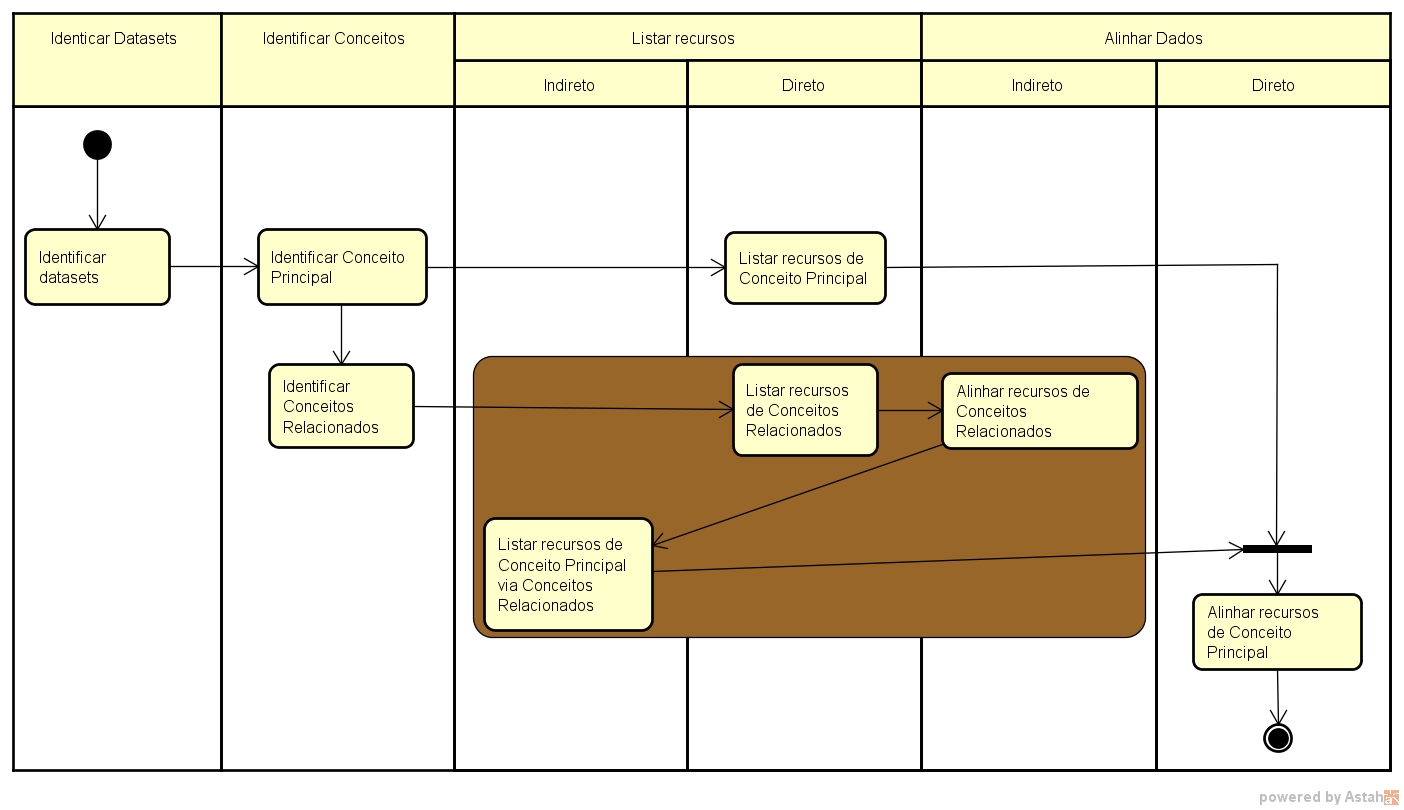
\includegraphics[width=0.9\textwidth]{./imagens/processo.png}
    \caption{Processo de alinhamento de dados conectados}
	\label{fig:processo}
\end{figure}

\section*{I - Selecionar Datasets}
A etapa de selecionar datasets trata da determinação de quais conjuntos de dados serão alinhados. A seleção de um dataset está sujeita a alguns critérios, tais como: estar estruturado em triplas e utilizar conceitos modelados em ontologias/vocabulários. Tais critérios foram determinados de acordo com o escopo do processo, pois este está limitado à dados conectados. Além de se adequar ao escopo, os critérios cumprem os requisitos mínimos para a execução do processo.
Complementarmente, a comunidade já disponibiliza ferramentas e processos para a publicação de dados conectados na Web, o que não é o foco desse processo. Além disso, é importante destacar que ao modelar os dados em qualquer processo de publicação de dados conectados são utilizadas ontologias/vocabulários que podem servir como base.

\section*{II - Identificar Conceitos}
A identificação de conceitos é dividida em duas atividades, uma automática e outra manual. A atividade automática se trata de recuperar os conceitos presentes na base de dados através de queries SPARQL que podem ser vistas a seguir.
\\
\begin{lstlisting}[captionpos=b, caption=Query SPARQL para identificação de conceito, label=lst:sparql,
   basicstyle=\ttfamily,frame=single]
PREFIX rdf: <http://www.w3.org/1999/02/22-rdf-syntax-ns#>
PREFIX rdfs: <http://www.w3.org/2000/01/rdf-schema#>
select distinct ?Concept count(*) as ?count where {
	[] 	a ?Concept.
	?Concept 	(^rdfs:domain|^rdfs:range) ?o.
}
group 	by ?Concept	
order 	by desc(?count)
\end{lstlisting}

Como resultado do Código \ref{lst:sparql} é apresentada uma lista contendo conceitos presentes na base, os conceitos estão ordenados decrescentemente de acordo com o número de recursos presentes na base. Neste momento, o usuário deve escolher que conceito deve ser alinhado. Após a seleção do conceito, será executada uma nova query SPARQL (ver Código \ref{lst:sparql2}), cujo objetivo é recuperar os conceitos relacionados ao conceito principal, que utiliza a escolha do usuário como parâmetro para a identificação.

\begin{lstlisting}[captionpos=b, caption=Query SPARQL para recuperação de conceitos relacionados, label=lst:sparql2,
   basicstyle=\ttfamily,frame=single]
PREFIX rdf: <http://www.w3.org/1999/02/22-rdf-syntax-ns#>
PREFIX rdfs: <http://www.w3.org/2000/01/rdf-schema#>


select distinct ?type where {
	values ?Concept{<URI do conceito escolhido>}
	{
		?instance rdf:type ?Concept; ?p ?o.
		?p rdf:type owl:ObjectProperty.
		?o rdf:type ?type.
	}
	union
	{
		?s ?p ?o.
		?p rdf:type owl:ObjectProperty.
		?o rdf:type ?Concept.
		?s rdf:type ?type.
	}
}

\end{lstlisting}

Como resultado do Código \ref{lst:sparql2} é provida uma lista contendo os conceitos relacionados ao conceito escolhido. Neste momento, o usuário deve escolher, quais conceitos relacionados ele deseja utilizar para melhorar o alinhamento do conceito escolhido. Tal decisão influenciará tanto no tempo que o processo levará para concluir, quanto na quantidade de recursos alinhados ao final do processo, pois para cada conceito relacionado haverá uma nova execução das etapas (iii) e (iv). Esse loop é necessário, pois alguns alinhamentos serão possíveis apenas através da relação entre esses conceitos.

\section*{III - Listar recursos}
A etapa de listar recursos pode ser entendida como a recuperação dos recursos que pertencem aos conceitos. É importante destacar que a listagem/recuperação de recursos da base de conhecimento pode ser executada mais de uma vez durante o processo, gerando um conjunto de recursos para cada conceito escolhido.


\section*{IV - Alinhar Dados}
A etapa de alinhamento de dados está dividida em duas atividades sendo elas alinhamento dos recursos e melhoramento. A atividade de alinhamento é composta de vários momentos, sendo eles: tratamento dos dados, comparação entre recursos e análise de similaridade.
No tratamento dos dados é aplicado um conjunto de transformações nas propriedades dos recursos, das quais podemos citar: deixar letras em minúsculos, remover pontos, acentuação.
Na comparação as propriedades dos recursos são comparadas entre si (ver Figura \ref{fig:resources}) através de algoritmos de similaridade de texto. Além disso, essas similaridades são utilizadas para a definição da similaridade entre recursos. Na análise de similaridade os resultados são comparados a um limiar de aceitação definido por um especialista no início do processo.

\begin{figure}[!ht]
	\centering
	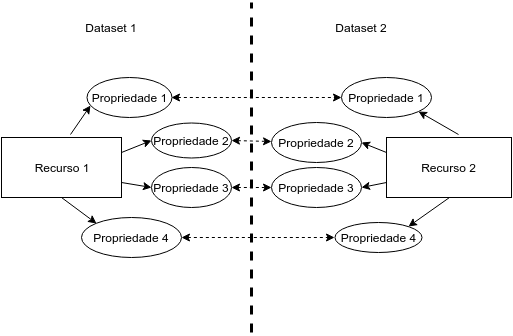
\includegraphics[width=0.7\textwidth]{./imagens/resources.png}
    \caption{Comparação entre recursos}
	\label{fig:resources}
\end{figure}